\documentclass[11pt,a4paper,oneside]{book}
%-- coding: UTF-8 --
\usepackage[UTF8]{ctex}
\usepackage{fontspec}
\defaultfontfeatures{Mapping=tex-text}
\usepackage{xunicode}
\usepackage{xltxtra}
\usepackage{amsmath}
\usepackage{amsfonts}
\usepackage{amssymb}
\usepackage{graphicx}
\usepackage{amsthm}
\usepackage{array}
\usepackage{float}   %{H}
\usepackage{booktabs}  %\toprule[1.5pt]
\setcounter{secnumdepth}{4}
\usepackage{indentfirst} %首行缩进
\usepackage{tcolorbox} %彩色框框
\usepackage{graphicx}  %图片并排
\usepackage{subfigure} %图片并排
\usepackage{graphicx} %插入jpg
\setcounter{secnumdepth}{4}		%增加编号深度
\setcounter{tocdepth}{4}		%增加目录深度
\usepackage{hyperref}     %生成pdf书签
\hypersetup{hidelinks,
	colorlinks=true,
	allcolors=black,
	pdfstartview=Fit,
	breaklinks=true
}       %去掉目录的红色框框
%===================%插入代码需要的控制
\usepackage{listings}
\usepackage{xcolor}
\setmonofont{Consolas}%字体
\lstset{
	numbers=left, 
	numberstyle= \tiny, 
	keywordstyle= \color{ blue!70},
	commentstyle= \color{red!50!green!50!blue!50}, 
	frame=shadowbox, % 阴影效果
	rulesepcolor= \color{ red!20!green!20!blue!20} ,
	escapeinside=``,% 英文分号中可写入中文
	breaklines      =   true, 
	basicstyle=\ttfamily 
} 
%===================%
\usepackage[left=2cm,right=2cm,top=2cm,bottom=2cm]{geometry}
\newtheorem{theorem}{定理}
\newtheorem{definition}{定义}
\pagestyle{plain}%设置页码
\title{\huge NOTE on SQL}
\author{zy}
\date{\today}

\begin{document}
	\maketitle
	\tableofcontents  %目录

\chapter{了解SQL}
\section{数据库基础}
\subsection{数据库}
数据库是一个以某种有组织的方式储存的数据集合.可以简单理解为一个文件柜,这个文件柜是存放数据的物理位置,不论数据为何,不论数据如何组织.
\begin{tcolorbox}[colback=blue!7!white,colframe=blue!40]
\textbf{数据库(database)}: 保存有组织的数据的容器(通常是一个文件或者一组文件)
\end{tcolorbox}
\begin{tcolorbox}[colback=pink!10!white,colframe=pink!100!black]
数据库软件应称为数据库管理系统(DBMS).数据库是通过DBMS创建和操纵的容器,而具体他究竟是什么,形式如何,各种数据库都不一样.
\end{tcolorbox}

\subsection{表}
往文件柜里放资料时,并不是随便将它们扔进某个抽屉就完事,而是在文件柜中创建文件,然后将相关的资料放入特定的文件中.

在数据库中,这种文件称为表.
\begin{tcolorbox}[colback=blue!7!white,colframe=blue!40]
\textbf{表(table)}: 某种特定类型数据的结构化清单
\end{tcolorbox}
表可以用来存储特定类型的数据.表可以保存顾客清单,产品目录,或者其他信息清单.

关键:储存在表中的数据时同一种类型的数据或清单,绝不应该将顾客的清单与订单的清单存储在同一个数据库表中.

命名唯一,不能同名.
\begin{tcolorbox}[colback=pink!10!white,colframe=pink!100!black]
使表名成为唯一的,实际上是数据库名和表名等的组合.有的数据库还使用数据库拥有者的名字作为唯一名的一部分.也就是说,虽然在相同的数据库中不能两次使用相同表名,但是在不同的数据库中完全可以.
\end{tcolorbox}
表具有一些特性,这些特性定义了数据在表中如何储存,包含存储什么样的数据,数据如何分解,各部分信息如何命名等信息.描述表的这组信息就是模式.
\begin{tcolorbox}[colback=blue!7!white,colframe=blue!40]
	\textbf{模式(schema)}: 关于数据库和表的布局及特性的信息.
\end{tcolorbox}
模式可以用来描述数据库中特定的表,也可以用来描述整个数据库(和其中表的关系).
\subsection{列和数据类型}
表由列组成.列存储表中某部分信息.
\begin{tcolorbox}[colback=blue!7!white,colframe=blue!40]
	\textbf{列(column)}: 表中的一个字段.所有表都是由一个或者多个列组成的.
\end{tcolorbox}
理解列最好的办法集是将数据库表想象出一个网格,网格中每一列存储着某种特定的信息.
\begin{tcolorbox}[colback=pink!10!white,colframe=pink!100!black]
分解数据

正确地将数据分解为多个列极为重要.如城市,州,邮政编码应该是彼此独立的列.通过分解这些数据,才有可能利用特定的列对数据进行分类和过滤(如找出特定州或特定城市的所有顾客).如果城市和州组合在一个列,则按州进行分类或过滤就会很困难.

你可以根据自己的具体需求来决定把数据分解到何种程度.
\end{tcolorbox}

数据库中每个列都有相应的数据类型.数据类型定义了列可以存储哪些数据种类.
\begin{tcolorbox}[colback=blue!7!white,colframe=blue!40]
\textbf{数据类型(datatype)}: 所允许的数据的类型.每个表列都有相应的数据类型,它限制或允许该列中存储的数据.
\end{tcolorbox}
数据类型还帮助正确地分类数据,并在优化磁盘使用方面起到重要作用.因此在创建表时必须特别关注所用的数据类型.
\begin{tcolorbox}[colback=pink!10!white,colframe=pink!100!black]
数据类型及其名称是SQL不兼容的一个主要原因.虽然大多数基本数据类型得到了一致的支持,但是许多高级的数据类型却没有.更糟的是,偶然会有相同的数据类型在不同的DBMS中具有不同的名称.对此用户你能咋地,重要的是在创建表结构时要记住这些差异.
\end{tcolorbox}
\subsection{行}
表中的数据是按行储存的,所保存的每个记录存储在自己的行内.如果将表想象为网络,网格中垂直的列为表列,水平行为表行.
\begin{tcolorbox}[colback=blue!7!white,colframe=blue!40]
\textbf{行(row)}: 表中的一个记录.
\end{tcolorbox}
\begin{tcolorbox}[colback=pink!10!white,colframe=pink!100!black]
用户在提到行时称其为数据库记录(record).这两个术语多半交替使用,行才是正确术语.
\end{tcolorbox}
\subsection{主键}
表中每一行都应该有一列(或几列)可以唯一标识自己.如雇员表的雇员id.
\begin{tcolorbox}[colback=blue!7!white,colframe=blue!40]
\textbf{主键(primary key)}: 一列,或一组列,其值可以唯一标识表中每一行.
\end{tcolorbox}
没有主键,更新或者删除表中特定行就极为困难,因为你不能保证操作只涉及相关的行.
\begin{tcolorbox}[colback=pink!10!white,colframe=pink!100!black]
虽然并不总是需要主键,但多数数据库设计者都会保证他们创建的每个表都具有一个主键,以便日后数据操作和管理.
\end{tcolorbox}
表中任意列都可以作为主键,只要满足以下条件:
\begin{itemize}
	\item 任意两行都不具有相同的主键值;
	\item 每一行都必须具有一个主键值(主键列不允许NULL值);
	\item 主键列的值不允许修改/更新;
	\item 主键值不能重用(如果某行从表中删除,它的主键不能赋给以后的新行).
\end{itemize}
在使用多列作为主键时,上述条件必须应用到所有列,所有列的组合必须是唯一的(但单个列的值可以不唯一).
\section{什么是SQL}
SQL是structured query language(结构化查询语言)的缩写.一种专门用来与数据库沟通的语言.

优点:
\begin{itemize}
	\item 几乎所有重要的DBMS都支持SQL.
	\item 简单易学.
	\item 语言强有力.
\end{itemize}
\begin{tcolorbox}[colback=pink!10!white,colframe=pink!100!black]
许多DBMS厂商对SQL进行了扩展,目的是提供执行特定操作的额外功能或简化方法,但一般针对个别DBMS.本书使用ANSI标准委员会管理的标准SQL,称ANSI SQL.
\end{tcolorbox}

\section{sql的启动/运行}

\begin{lstlisting}[language=sql]
C:\Windows\system32>net start mysql
MySQL 服务正在启动 .
MySQL 服务已经启动成功。
\end{lstlisting}
创建和填充书中各章所用的表:
\begin{lstlisting}[language=sql]
C:\Windows\system32>mysql -uroot -proot

mysql> create database crashcourse;

mysql> use crashcourse;

mysql> source D:\mysql_scripts\create.sql 

mysql> source D:\mysql_scripts\populate.sql

\end{lstlisting}

\chapter{检索数据}
\begin{figure}[H]
	\centering
	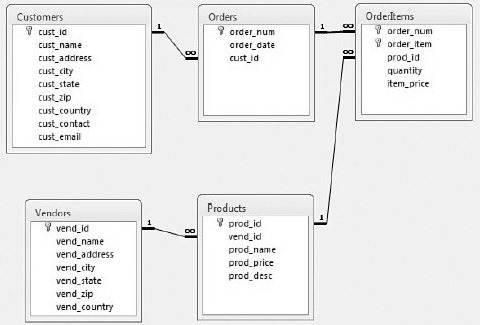
\includegraphics[width=\textwidth]{1.png}
\end{figure}
\section{SELECT语句}
\begin{tcolorbox}[colback=blue!7!white,colframe=blue!40]
	\textbf{关键字(keyword)}
	作为SQL 组成部分的保留字。关键字不能用作表或列的名字。附录E列出了某些经常使用的保留字。
\end{tcolorbox}
SELECT 语句的用途:从一个或多个表中检索信息,将返回表中的所有行。

\section{检索单个列}
\begin{lstlisting}[language=sql]
mysql> SELECT prod_name
-> FROM Products;
+----------------+
| prod_name      |
+----------------+
| .5 ton anvil   |
| 1 ton anvil    |
| 2 ton anvil    |
| Detonator      |
| Bird seed      |
| Carrots        |
| Fuses          |
| JetPack 1000   |
| JetPack 2000   |
| Oil can        |
| Safe           |
| Sling          |
| TNT (1 stick)  |
| TNT (5 sticks) |
+----------------+
14 rows in set (0.02 sec)
\end{lstlisting}
如果没有明确排序查询结果(下一课介绍),则返回的数据没有特定的顺序。返回数据的顺序可能是数据被添加到表中的顺序,也可能不是。只要返回相同数目的行,就是正常的。

请注意,SQL语句不区分大小写,因此SELECT 与select 是相同的。在处理SQL 语句时,其中所有空格都被忽略。SQL 语句可以写成长长
的一行,也可以分写在多行。下面这3 种写法的作用是一样的。
\begin{lstlisting}[language=sql]
SELECT prod_name
FROM Products;

SELECT prod_name FROM Products;

SELECT
prod_name
FROM
Products;	
\end{lstlisting}
多数SQL 开发人员认为,将SQL 语句分成多行更容易阅读和调试。

\section{检索多个列}
在选择多个列时,一定要在列名之间加上逗号,但最后一个列名后不加。如果在最后一个列名后加了逗号,将出现错误
\begin{lstlisting}[language=sql]
mysql> select prod_id,prod_name,prod_price
-> from products;
+---------+----------------+------------+
| prod_id | prod_name      | prod_price |
+---------+----------------+------------+
| ANV01   | .5 ton anvil   |       5.99 |
| ANV02   | 1 ton anvil    |       9.99 |
| ANV03   | 2 ton anvil    |      14.99 |
| DTNTR   | Detonator      |      13.00 |
| FB      | Bird seed      |      10.00 |
| FC      | Carrots        |       2.50 |
| FU1     | Fuses          |       3.42 |
| JP1000  | JetPack 1000   |      35.00 |
| JP2000  | JetPack 2000   |      55.00 |
| OL1     | Oil can        |       8.99 |
| SAFE    | Safe           |      50.00 |
| SLING   | Sling          |       4.49 |
| TNT1    | TNT (1 stick)  |       2.50 |
| TNT2    | TNT (5 sticks) |      10.00 |
+---------+----------------+------------+
14 rows in set (0.01 sec)
\end{lstlisting}
SQL 语句一般返回原始的、无格式的数据。数据的格式化是表示问题,而不是检索问题。因此,表示(如把上面的价格值显示为正确的十进制数值货币金额)一般在显示该数据的应用程序中规定。通常很少直接使用实际检索出的数据(没有应用程序提供的格式)。

\section{检索所有列}
如果给定一个通配符(*),则返回表中所有列。列的顺序一般是列在表定义中出现的物理顺序,但并不总是如此。

一般而言,除非你确实需要表中的每一列,否则最好别使用*通配符。
\begin{lstlisting}[language=sql]
mysql> select *
-> from products;
+---------+---------+----------------+------------+----------------------------------------
| prod_id | vend_id | prod_name      | prod_price | prod_desc 
+---------+---------+----------------+------------+----------------------------------------
| ANV01   |    1001 | .5 ton anvil   |       5.99 | .5 ton anvil, black...
| ANV02   |    1001 | 1 ton anvil    |       9.99 | 1 ton anvil, black...
| ANV03   |    1001 | 2 ton anvil    |      14.99 | 2 ton anvil, black...
| DTNTR   |    1003 | Detonator      |      13.00 | Detonator (plunger ...
| FB      |    1003 | Bird seed      |      10.00 | Large bag (suitable ...
| FC      |    1003 | Carrots        |       2.50 | Carrots (rabbit...
| FU1     |    1002 | Fuses          |       3.42 | 1 dozen, extra long...
| JP1000  |    1005 | JetPack 1000   |      35.00 | JetPack 1000, intended...
| JP2000  |    1005 | JetPack 2000   |      55.00 | JetPack 2000, multi-use...
| OL1     |    1002 | Oil can        |       8.99 | Oil can, red...
| SAFE    |    1003 | Safe           |      50.00 | Safe with combination...
| SLING   |    1003 | Sling          |       4.49 | Sling, one size fits...
| TNT1    |    1003 | TNT (1 stick)  |       2.50 | TNT, red, single...
| TNT2    |    1003 | TNT (5 sticks) |      10.00 | TNT, red, pack of 10...
+---------+---------+----------------+------------+----------------------------------------
14 rows in set (0.01 sec)
\end{lstlisting}
使用通配符有一个大优点。由于不明确指定列名(因为星号检索每一列),所以能检索出名字未知的列。

\section{检索不同的值}
SELECT 语句返回所有匹配的行。但是,如果你不希望每个值每次都出现,该怎么办呢?例如,你想检索products 表中所有产品供应商的ID:
\begin{lstlisting}[language=sql]
mysql> select vend_id
-> from products;
+---------+
| vend_id |
+---------+
|    1001 |
|    1001 |
|    1001 |
|    1002 |
|    1002 |
|    1003 |
|    1003 |
|    1003 |
|    1003 |
|    1003 |
|    1003 |
|    1003 |
|    1005 |
|    1005 |
+---------+
14 rows in set (0.01 sec)
\end{lstlisting}
SELECT 语句返回14行(即使表中只有4个产品供应商),因为products表中有14种产品。那么如何检索出不同的值?办法就是使用DISTINCT 关键字,顾名思义,它指示数据库只返回不同的值。
\begin{lstlisting}[language=sql]
mysql> select distinct vend_id
-> from products;
+---------+
| vend_id |
+---------+
|    1001 |
|    1002 |
|    1003 |
|    1005 |
+---------+
4 rows in set (0.02 sec)
\end{lstlisting}
\begin{tcolorbox}[colback=pink!10!white,colframe=pink!100!black]
\textbf{注意:不能部分使用DISTINCT}
DISTINCT 关键字作用于所有的列,不仅仅是跟在其后的那一列。例如,你指定SELECT DISTINCT vend\_id, prod\_price,除非指定的两列完全相同,否则所有的行都会被检索出来。
\end{tcolorbox}

\section{限制结果}
如果你只想返回第一行或者一定数量的行,该怎么办呢?这是可行的,然而遗憾的是,各种数据库中的这一SQL 实现并不相同。

LIMIT 5 指示MySQL等DBMS 返回不超过5 行的数据。
\begin{lstlisting}[language=sql]
mysql> select prod_name
-> from products
-> limit 5;
+--------------+
| prod_name    |
+--------------+
| .5 ton anvil |
| 1 ton anvil  |
| 2 ton anvil  |
| Detonator    |
| Bird seed    |
+--------------+
5 rows in set (0.01 sec)
\end{lstlisting}

为了得到后面的5 行数据,需要指定从哪儿开始以及检索的行数,像这样:
\begin{lstlisting}[language=sql]
mysql> select prod_name
-> from products
-> limit 5 offset 5;
+--------------+
| prod_name    |
+--------------+
| Carrots      |
| Fuses        |
| JetPack 1000 |
| JetPack 2000 |
| Oil can      |
+--------------+
5 rows in set (0.00 sec)
\end{lstlisting}
LIMIT 5 OFFSET 5 指示MySQL 等DBMS 返回从第5 行起的5 行数据。
第一个数字是指从哪儿开始,第二个数字是检索的行数。所以,LIMIT 指定返回的行数。LIMIT 带的OFFSET 指定从哪儿开始。

\begin{tcolorbox}[colback=pink!10!white,colframe=pink!100!black]
\textbf{注意:第0 行}

第一个被检索的行是第0 行,而不是第1 行。因此,LIMIT 1 OFFSET
1 会检索第2 行,而不是第1 行。
\end{tcolorbox}

\section{使用注释}
注释使用-- (两个连字符)嵌在行内。-- 之后的文本就是注释.

在一行的开始处使用\#,这一整行都将作为注释.

注释从/*开始,到*/结束,/*和*/之间的任何内容都是注释。

\chapter{排序检索数据}
\section{排序数据}
下面的SQL 语句返回某个数据库表的单个列。但请看
其输出,并没有特定的顺序。
\begin{lstlisting}[language=sql]
mysql> select prod_name
-> from products;
+----------------+
| prod_name      |
+----------------+
| .5 ton anvil   |
| 1 ton anvil    |
| 2 ton anvil    |
| Detonator      |
| Bird seed      |
| Carrots        |
| Fuses          |
| JetPack 1000   |
| JetPack 2000   |
| Oil can        |
| Safe           |
| Sling          |
| TNT (1 stick)  |
| TNT (5 sticks) |
+----------------+
14 rows in set (0.00 sec)
\end{lstlisting}
其实,检索出的数据并不是随机显示的。如果不排序,数据一般将以它在底层表中出现的顺序显示,这有可能是数据最初添加到表中的顺序。但是,如果数据随后进行过更新或删除,那么这个顺序将会受到DBMS 重用回收存储空间的方式的影响。因此,如果不明确控制的话,则最终的结果不能(也不应该)依赖该排序顺序。关系数据库设计理论认为,如果不明确规定排序顺序,则不应该假定检索出的数据的顺序有任何意义。

\begin{tcolorbox}[colback=pink!10!white,colframe=pink!100!black]
\textbf{子句(clause)}
SQL 语句由子句构成,有些子句是必需的,有些则是可选的。一个子句通常由一个关键字加上所提供的数据组成。子句的例子有我们在前一课看到的SELECT 语句的FROM 子句。
\end{tcolorbox}

为了明确地排序用SELECT 语句检索出的数据,可使用ORDER BY 子句。
ORDER BY 子句取一个或多个列的名字,据此对输出进行排序。请看下面
的例子:

\begin{lstlisting}[language=sql]
mysql> select prod_name
-> from products
-> order by prod_name;
+----------------+
| prod_name      |
+----------------+
| .5 ton anvil   |
| 1 ton anvil    |
| 2 ton anvil    |
| Bird seed      |
| Carrots        |
| Detonator      |
| Fuses          |
| JetPack 1000   |
| JetPack 2000   |
| Oil can        |
| Safe           |
| Sling          |
| TNT (1 stick)  |
| TNT (5 sticks) |
+----------------+
14 rows in set (0.01 sec)
\end{lstlisting}
除了指示DBMS 软件对prod\_name 列以字母顺序排序数据的ORDER BY子句外,这条语句与前面的语句相同.

通常,ORDER BY 子句中使用的列将是为显示而选择的列。但是,实际上并不一定要这样,用非检索的列排序数据是完全合法的。

\section{按多个列排序}
经常需要按不止一个列进行数据排序。例如,如果要显示雇员名单,可能希望按姓和名排序(首先按姓排序,然后在每个姓中再按名排序)。如果多个雇员有相同的姓,这样做很有用。

要按多个列排序,简单指定列名,列名之间用逗号分开即可(就像选择多个列时那样).
\begin{lstlisting}[language=sql]
mysql> select prod_id,prod_price,prod_name
-> from products
-> ;
+---------+------------+----------------+
| prod_id | prod_price | prod_name      |
+---------+------------+----------------+
| ANV01   |       5.99 | .5 ton anvil   |
| ANV02   |       9.99 | 1 ton anvil    |
| ANV03   |      14.99 | 2 ton anvil    |
| DTNTR   |      13.00 | Detonator      |
| FB      |      10.00 | Bird seed      |
| FC      |       2.50 | Carrots        |
| FU1     |       3.42 | Fuses          |
| JP1000  |      35.00 | JetPack 1000   |
| JP2000  |      55.00 | JetPack 2000   |
| OL1     |       8.99 | Oil can        |
| SAFE    |      50.00 | Safe           |
| SLING   |       4.49 | Sling          |
| TNT1    |       2.50 | TNT (1 stick)  |
| TNT2    |      10.00 | TNT (5 sticks) |
+---------+------------+----------------+
14 rows in set (0.00 sec)
\end{lstlisting}
\begin{lstlisting}[language=sql]
mysql> select prod_id,prod_price,prod_name
-> from products
-> order by prod_price,prod_name;
+---------+------------+----------------+
| prod_id | prod_price | prod_name      |
+---------+------------+----------------+
| FC      |       2.50 | Carrots        |
| TNT1    |       2.50 | TNT (1 stick)  |
| FU1     |       3.42 | Fuses          |
| SLING   |       4.49 | Sling          |
| ANV01   |       5.99 | .5 ton anvil   |
| OL1     |       8.99 | Oil can        |
| ANV02   |       9.99 | 1 ton anvil    |
| FB      |      10.00 | Bird seed      |
| TNT2    |      10.00 | TNT (5 sticks) |
| DTNTR   |      13.00 | Detonator      |
| ANV03   |      14.99 | 2 ton anvil    |
| JP1000  |      35.00 | JetPack 1000   |
| SAFE    |      50.00 | Safe           |
| JP2000  |      55.00 | JetPack 2000   |
+---------+------------+----------------+
14 rows in set (0.00 sec)
\end{lstlisting}
对于上述例子中的输出,仅在多个行具有相同的prod\_price 值时
才对产品按prod\_name 进行排序。如果prod\_price 列中所有的值都是
唯一的,则不会按prod\_name 排序。

\section{按列位置排序}
除了能用列名指出排序顺序外,ORDER BY 还支持按相对列位置进行排序。
\begin{lstlisting}[language=sql]
mysql> select prod_id,prod_price,prod_name
-> from products
-> order by 2,3;
+---------+------------+----------------+
| prod_id | prod_price | prod_name      |
+---------+------------+----------------+
| FC      |       2.50 | Carrots        |
| TNT1    |       2.50 | TNT (1 stick)  |
| FU1     |       3.42 | Fuses          |
| SLING   |       4.49 | Sling          |
| ANV01   |       5.99 | .5 ton anvil   |
| OL1     |       8.99 | Oil can        |
| ANV02   |       9.99 | 1 ton anvil    |
| FB      |      10.00 | Bird seed      |
| TNT2    |      10.00 | TNT (5 sticks) |
| DTNTR   |      13.00 | Detonator      |
| ANV03   |      14.99 | 2 ton anvil    |
| JP1000  |      35.00 | JetPack 1000   |
| SAFE    |      50.00 | Safe           |
| JP2000  |      55.00 | JetPack 2000   |
+---------+------------+----------------+
14 rows in set (0.01 sec)
\end{lstlisting}
可以看到,这里的输出与上面的查询相同,不同之处在于ORDER BY 子句。SELECT 清单中指定的是选择列的相对位置而不是列名。ORDER BY 2表示按SELECT 清单中的第二个列prod\_name 进行排序。ORDER BY 2,3表示先按prod\_price,再按prod\_name 进行排序。

这一技术的主要好处在于不用重新输入列名。但它也有缺点。首先,不明确给出列名有可能造成错用列名排序。其次,在对SELECT 清单进行更改时容易错误地对数据进行排序(忘记对ORDER BY 子句做相应的改动)。最后,如果进行排序的列不在SELECT 清单中,显然不能使用这项技术。
\section{指定排序方向}
数据排序不限于升序排序(从A 到Z),这只是默认的排序顺序。还可以使用ORDER BY 子句进行降序(从Z 到A)排序。为了进行降序排序,必须指定DESC 关键字。

下面的例子以价格降序来排序产品(最贵的排在最前面):

\begin{lstlisting}[language=sql]
mysql> select prod_id,prod_price,prod_name
-> from products
-> order by prod_price desc;
+---------+------------+----------------+
| prod_id | prod_price | prod_name      |
+---------+------------+----------------+
| JP2000  |      55.00 | JetPack 2000   |
| SAFE    |      50.00 | Safe           |
| JP1000  |      35.00 | JetPack 1000   |
| ANV03   |      14.99 | 2 ton anvil    |
| DTNTR   |      13.00 | Detonator      |
| FB      |      10.00 | Bird seed      |
| TNT2    |      10.00 | TNT (5 sticks) |
| ANV02   |       9.99 | 1 ton anvil    |
| OL1     |       8.99 | Oil can        |
| ANV01   |       5.99 | .5 ton anvil   |
| SLING   |       4.49 | Sling          |
| FU1     |       3.42 | Fuses          |
| FC      |       2.50 | Carrots        |
| TNT1    |       2.50 | TNT (1 stick)  |
+---------+------------+----------------+
14 rows in set (0.00 sec)
\end{lstlisting}

如果打算用多个列排序,该怎么办?下面的例子以降序排序产品(最贵的在最前面),再加上产品名:
\begin{lstlisting}[language=sql]
mysql> select prod_id,prod_price,prod_name
-> from products
-> order by prod_price desc,prod_name;
+---------+------------+----------------+
| prod_id | prod_price | prod_name      |
+---------+------------+----------------+
| JP2000  |      55.00 | JetPack 2000   |
| SAFE    |      50.00 | Safe           |
| JP1000  |      35.00 | JetPack 1000   |
| ANV03   |      14.99 | 2 ton anvil    |
| DTNTR   |      13.00 | Detonator      |
| FB      |      10.00 | Bird seed      |
| TNT2    |      10.00 | TNT (5 sticks) |
| ANV02   |       9.99 | 1 ton anvil    |
| OL1     |       8.99 | Oil can        |
| ANV01   |       5.99 | .5 ton anvil   |
| SLING   |       4.49 | Sling          |
| FU1     |       3.42 | Fuses          |
| FC      |       2.50 | Carrots        |
| TNT1    |       2.50 | TNT (1 stick)  |
+---------+------------+----------------+
14 rows in set (0.00 sec)
\end{lstlisting}
DESC 关键字只应用到直接位于其前面的列名.如果想在多个列上进行降序排序,必须对每一列指定DESC 关键字。

请注意,DESC 是DESCENDING 的缩写,这两个关键字都可以使用。与DESC相对的是ASC(或ASCENDING),在升序排序时可以指定它。但实际上,ASC 没有多大用处,因为升序是默认的.

\chapter{过滤数据}
这一课将讲授如何使用SELECT 语句的WHERE 子句指定搜索条件。
\section{使用where子句}
数据库表一般包含大量的数据,很少需要检索表中的所有行。通常只会
根据特定操作或报告的需要提取表数据的子集。只检索所需数据需要指
定\textbf{搜索条件(search criteria)},搜索条件也称为\textbf{过滤条件(filter condition)}。

在SELECT 语句中,数据根据WHERE 子句中指定的搜索条件进行过滤。WHERE 子句在表名(FROM 子句)之后给出,如下所示:
\begin{lstlisting}[language=sql]
mysql> select prod_name,prod_price
-> from products
-> where prod_price=3.42;
+-----------+------------+
| prod_name | prod_price |
+-----------+------------+
| Fuses     |       3.42 |
+-----------+------------+
1 row in set (0.01 sec)
\end{lstlisting}
在同时使用ORDER BY 和WHERE 子句时,应该让ORDER BY 位于WHERE 之后,否则将会产生错误.

\section{where子句操作符}
\begin{figure}[H]
	\centering
	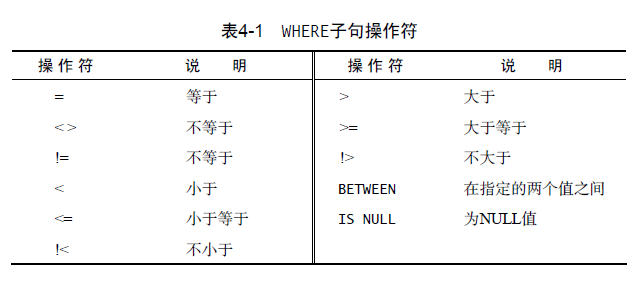
\includegraphics[width=0.8\textwidth]{2.png}
\end{figure}
表4-1 中列出的某些操作符是冗余的(如< >与!=相同,!<相当于>=)。并非所有DBMS 都支持这些操作符。想确定你的DBMS 支持哪些操作符,请参阅相应的文档。

\subsection{检查单个值}
我们已经看到了检验相等的例子,现在来看看几个使用其他操作符的例子。第一个例子是列出所有价格小于10 美元的产品。
\begin{lstlisting}[language=sql]
mysql> select prod_name,prod_price
-> from products
-> where prod_price<10;
+---------------+------------+
| prod_name     | prod_price |
+---------------+------------+
| .5 ton anvil  |       5.99 |
| 1 ton anvil   |       9.99 |
| Carrots       |       2.50 |
| Fuses         |       3.42 |
| Oil can       |       8.99 |
| Sling         |       4.49 |
| TNT (1 stick) |       2.50 |
+---------------+------------+
7 rows in set (0.01 sec)
\end{lstlisting}
下一条语句检索所有价格小于等于10 美元的产品
\begin{lstlisting}[language=sql]
mysql> select prod_name,prod_price
-> from products
-> where prod_price<=10;
+----------------+------------+
| prod_name      | prod_price |
+----------------+------------+
| .5 ton anvil   |       5.99 |
| 1 ton anvil    |       9.99 |
| Bird seed      |      10.00 |
| Carrots        |       2.50 |
| Fuses          |       3.42 |
| Oil can        |       8.99 |
| Sling          |       4.49 |
| TNT (1 stick)  |       2.50 |
| TNT (5 sticks) |      10.00 |
+----------------+------------+
9 rows in set (0.00 sec)
\end{lstlisting}

\subsection{检查单个值}
列出所有不是1003供应商制造的产品:
\begin{lstlisting}[language=sql]
mysql> select vend_id,prod_name
-> from products
-> where vend_id<>'1003';
+---------+--------------+
| vend_id | prod_name    |
+---------+--------------+
|    1001 | .5 ton anvil |
|    1001 | 1 ton anvil  |
|    1001 | 2 ton anvil  |
|    1002 | Fuses        |
|    1002 | Oil can      |
|    1005 | JetPack 1000 |
|    1005 | JetPack 2000 |
+---------+--------------+
7 rows in set (0.01 sec)
\end{lstlisting}
\begin{tcolorbox}[colback=pink!10!white,colframe=pink!100!black]
\textbf{提示:何时使用引号}

如果仔细观察上述WHERE 子句中的条件,会看到有的值括在单引号内,
而有的值未括起来。单引号用来限定字符串。如果将值与字符串类型的
列进行比较,就需要限定引号。用来与数值列进行比较的值不用引号。
\end{tcolorbox}
下面是相同的例子,其中使用!=而不是<>操作符:
\begin{lstlisting}[language=sql]
mysql> select vend_id,prod_name
-> from products
-> where vend_id!='1003';
+---------+--------------+
| vend_id | prod_name    |
+---------+--------------+
|    1001 | .5 ton anvil |
|    1001 | 1 ton anvil  |
|    1001 | 2 ton anvil  |
|    1002 | Fuses        |
|    1002 | Oil can      |
|    1005 | JetPack 1000 |
|    1005 | JetPack 2000 |
+---------+--------------+
7 rows in set (0.00 sec)
\end{lstlisting}

\subsection{范围值检查}
要检查某个范围的值,可以使用BETWEEN 操作符。其语法与其他WHERE子句的操作符稍有不同,因为它需要两个值,即范围的开始值和结束值。
\begin{lstlisting}[language=sql]
mysql> select prod_name,prod_price
-> from products
-> where prod_price between 5 and 10;
+----------------+------------+
| prod_name      | prod_price |
+----------------+------------+
| .5 ton anvil   |       5.99 |
| 1 ton anvil    |       9.99 |
| Bird seed      |      10.00 |
| Oil can        |       8.99 |
| TNT (5 sticks) |      10.00 |
+----------------+------------+
5 rows in set (0.01 sec)
\end{lstlisting}

\subsection{空值检查}
在创建表时,表设计人员可以指定其中的列能否不包含值。在一个列不包含值时,称其包含空值NULL。
\begin{tcolorbox}[colback=blue!7!white,colframe=blue!40]
	\textbf{NULL}
	
	无值(no value),它与字段包含0、空字符串或仅仅包含空格不同。
\end{tcolorbox}

确定值是否为NULL,不能简单地检查是否= NULL。SELECT 语句有一个
特殊的WHERE 子句,可用来检查具有NULL 值的列。这个WHERE 子句就
是IS NULL 子句。
\begin{lstlisting}[language=sql]
mysql> SELECT prod_name
-> from products
-> where prod_price is null;
Empty set (0.00 sec)
\end{lstlisting}
这条语句返回所有没有价格(空prod\_price 字段,不是价格为0)的
产品,由于表中没有这样的行,所以没有返回数据。

但是,Customers表确实包含具有NULL 值的列:如果没有电子邮件地址,则cust\_email
列将包含NULL 值:
\begin{lstlisting}[language=sql]
mysql> select cust_name
-> from customers
-> where cust_email is null;
+-------------+
| cust_name   |
+-------------+
| Mouse House |
| E Fudd      |
+-------------+
2 rows in set (0.00 sec)
\end{lstlisting}
\begin{tcolorbox}[colback=pink!10!white,colframe=pink!100!black]
\textbf{注意:NULL 和非匹配}

通过过滤选择不包含指定值的所有行时,你可能希望返回含NULL 值
的行。但是这做不到。因为未知(unknown)有特殊的含义,数据库
不知道它们是否匹配,所以在进行匹配过滤或非匹配过滤时,不会返
回这些结果。

过滤数据时,一定要验证被过滤列中含NULL 的行确实出现在返回的
数据中。
\end{tcolorbox}

\chapter{高级数据过滤}
\section{组合where子句}
为了进行更强的过滤控制,SQL允许给出多个WHERE 子句。这些子句有两种使用方式,即以AND 子句或OR 子句的方式使用。

\begin{tcolorbox}[colback=blue!7!white,colframe=blue!40]
\textbf{操作符(operator)}

用来联结或改变WHERE 子句中的子句的关键字,也称为逻辑操作符(logical operator)。
\end{tcolorbox}

\subsection{and操作符}
要通过不止一个列进行过滤,可以使用AND 操作符给WHERE 子句附加条件。下面的代码给出了一个例子:
\begin{lstlisting}[language=sql]
mysql> select prod_id,prod_price,prod_name
-> from products
-> where vend_id='1003'and prod_price<=4;
+---------+------------+---------------+
| prod_id | prod_price | prod_name     |
+---------+------------+---------------+
| FC      |       2.50 | Carrots       |
| TNT1    |       2.50 | TNT (1 stick) |
+---------+------------+---------------+
2 rows in set (0.01 sec)
\end{lstlisting}
\begin{tcolorbox}[colback=blue!7!white,colframe=blue!40]
	\textbf{and}
	
	用在WHERE 子句中的关键字,用来指示检索满足所有给定条件的行。
\end{tcolorbox}
这个例子只包含一个AND 子句,因此最多有两个过滤条件。可以增加多
个过滤条件,每个条件间都要使用AND 关键字。

\subsection{or操作符}
OR 操作符与AND 操作符正好相反,它指示DBMS 检索匹配任一条件的
行。事实上,许多DBMS 在OR WHERE 子句的第一个条件得到满足的情
况下,就不再计算第二个条件了(在第一个条件满足时,不管第二个条
件是否满足,相应的行都将被检索出来)。
\begin{lstlisting}[language=sql]
mysql> select prod_name,prod_price
-> from products
-> where vend_id='1003' or vend_id='1005';
+----------------+------------+
| prod_name      | prod_price |
+----------------+------------+
| Detonator      |      13.00 |
| Bird seed      |      10.00 |
| Carrots        |       2.50 |
| Safe           |      50.00 |
| Sling          |       4.49 |
| TNT (1 stick)  |       2.50 |
| TNT (5 sticks) |      10.00 |
| JetPack 1000   |      35.00 |
| JetPack 2000   |      55.00 |
+----------------+------------+
9 rows in set (0.00 sec)
\end{lstlisting}

\subsection{求值顺序}
WHERE 子句可以包含任意数目的AND 和OR 操作符。允许两者结合以进
行复杂、高级的过滤。
但是,组合AND 和OR 会带来了一个有趣的问题。为了说明这个问题,
来看一个例子。

\begin{lstlisting}[language=sql]
mysql> select prod_name,prod_price
-> from products
-> where vend_id='1003' or vend_id='1005'and prod_price>=10;
+----------------+------------+
| prod_name      | prod_price |
+----------------+------------+
| Detonator      |      13.00 |
| Bird seed      |      10.00 |
| Carrots        |       2.50 |
| Safe           |      50.00 |
| Sling          |       4.49 |
| TNT (1 stick)  |       2.50 |
| TNT (5 sticks) |      10.00 |
| JetPack 1000   |      35.00 |
| JetPack 2000   |      55.00 |
+----------------+------------+
9 rows in set (0.00 sec)
\end{lstlisting}
返回的行中有4 行价格小于10 美元,显然,返回的行
未按预期的进行过滤。为什么会这样呢?原因在于求值的顺序。SQL(像
多数语言一样)在处理OR 操作符前,优先处理AND 操作符。

它理解为:由供应商1005制造的价格为10 美元以
上的所有产品,以及由供应商1003制造的所有产品

此问题的解决方法是使用圆括号对操作符进行明确分组。请看下面的
SELECT 语句及输出:
\begin{lstlisting}[language=sql]
mysql> select prod_name,prod_price
-> from products
-> where(vend_id='1003' or vend_id='1005') and prod_price>=10;
+----------------+------------+
| prod_name      | prod_price |
+----------------+------------+
| Detonator      |      13.00 |
| Bird seed      |      10.00 |
| Safe           |      50.00 |
| TNT (5 sticks) |      10.00 |
| JetPack 1000   |      35.00 |
| JetPack 2000   |      55.00 |
+----------------+------------+
6 rows in set (0.01 sec)
\end{lstlisting}

\section{in操作符}
IN 操作符用来指定条件范围,范围中的每个条件都可以进行匹配。IN 取
一组由逗号分隔、括在圆括号中的合法值。
\begin{lstlisting}[language=sql]
mysql> select prod_name,prod_price
-> from products
-> where vend_id in('1003','1005')
-> order by prod_name;
+----------------+------------+
| prod_name      | prod_price |
+----------------+------------+
| Bird seed      |      10.00 |
| Carrots        |       2.50 |
| Detonator      |      13.00 |
| JetPack 1000   |      35.00 |
| JetPack 2000   |      55.00 |
| Safe           |      50.00 |
| Sling          |       4.49 |
| TNT (1 stick)  |       2.50 |
| TNT (5 sticks) |      10.00 |
+----------------+------------+
9 rows in set (0.00 sec)
\end{lstlisting}
IN 操作符完成了与OR 相同的功能.
\begin{lstlisting}[language=sql]
mysql> select prod_name,prod_price
-> from products
-> where vend_id='1003' or vend_id='1005'
-> order by prod_name;
+----------------+------------+
| prod_name      | prod_price |
+----------------+------------+
| Bird seed      |      10.00 |
| Carrots        |       2.50 |
| Detonator      |      13.00 |
| JetPack 1000   |      35.00 |
| JetPack 2000   |      55.00 |
| Safe           |      50.00 |
| Sling          |       4.49 |
| TNT (1 stick)  |       2.50 |
| TNT (5 sticks) |      10.00 |
+----------------+------------+
9 rows in set (0.00 sec)
\end{lstlisting}

为什么要使用IN 操作符?其优点如下。
\begin{itemize}
	\item 在有很多合法选项时,IN 操作符的语法更清楚,更直观。
	\item 在与其他AND 和OR 操作符组合使用IN 时,求值顺序更容易管理。
	\item IN 操作符一般比一组OR 操作符执行得更快(在上面这个合法选项很
	少的例子中,你看不出性能差异)。
	\item IN 的最大优点是可以包含其他SELECT 语句,能够更动态地建立
	WHERE 子句。第11 课会对此进行详细介绍。
\end{itemize}
\begin{tcolorbox}[colback=blue!7!white,colframe=blue!40]
	\textbf{IN}
	
	WHERE 子句中用来指定要匹配值的清单的关键字,功能与OR 相当。
\end{tcolorbox}

\section{not操作符}
WHERE 子句中的NOT 操作符有且只有一个功能,那就是否定其后所跟的
任何条件。因为NOT 从不单独使用(它总是与其他操作符一起使用),所
以它的语法与其他操作符有所不同。NOT 关键字可以用在要过滤的列前,
而不仅是在其后。
\begin{tcolorbox}[colback=blue!7!white,colframe=blue!40]
	\textbf{NOT}
	WHERE 子句中用来否定其后条件的关键字。
\end{tcolorbox}
下面的例子说明NOT 的用法。为了列出除1003 之外的所有供应商制造
的产品,可编写如下的代码。
\begin{lstlisting}[language=sql]
mysql> select prod_name
-> from products
-> where not vend_id='1003'
-> order by prod_name;
+--------------+
| prod_name    |
+--------------+
| .5 ton anvil |
| 1 ton anvil  |
| 2 ton anvil  |
| Fuses        |
| JetPack 1000 |
| JetPack 2000 |
| Oil can      |
+--------------+
7 rows in set (0.00 sec)
\end{lstlisting}
上面的例子也可以使用<>操作符来完成,如下所示。
\begin{lstlisting}[language=sql]
mysql> select prod_name
-> from products
-> where vend_id<>'1003'
-> order by prod_name;
+--------------+
| prod_name    |
+--------------+
| .5 ton anvil |
| 1 ton anvil  |
| 2 ton anvil  |
| Fuses        |
| JetPack 1000 |
| JetPack 2000 |
| Oil can      |
+--------------+
7 rows in set (0.00 sec)
\end{lstlisting}

为什么使用NOT?对于这里的这种简单的WHERE 子句,使用NOT 确实
没有什么优势。但在更复杂的子句中,NOT 是非常有用的。例如,在
与IN 操作符联合使用时,NOT 可以非常简单地找出与条件列表不匹配
的行。

\chapter{用通配符进行过滤}
这一课介绍什么是通配符、如何使用通配符以及怎样使用LIKE 操作符
进行通配搜索,以便对数据进行复杂过滤。

\section{like操作符}
前面介绍的所有操作符都是针对已知值进行过滤的。不管是匹配一个值
还是多个值,检验大于还是小于已知值,或者检查某个范围的值,其共
同点是过滤中使用的值都是已知的。

但是,这种过滤方法并不是任何时候都好用。例如,怎样搜索产品名中
包含文本bean bag 的所有产品?用简单的比较操作符肯定不行,必须使
用通配符。利用通配符,可以创建比较特定数据的搜索模式。

\begin{tcolorbox}[colback=blue!7!white,colframe=blue!40]
	\textbf{通配符(wildcard)}
	
	用来匹配值的一部分的特殊字符。
\end{tcolorbox}
\begin{tcolorbox}[colback=blue!7!white,colframe=blue!40]
	\textbf{搜索模式(search pattern)}
	
	由字面值、通配符或两者组合构成的搜索条件。
\end{tcolorbox}

通配符本身实际上是SQL 的WHERE 子句中有特殊含义的字符,SQL 支持
几种通配符。为在搜索子句中使用通配符,必须使用LIKE 操作符。LIKE
指示DBMS,后跟的搜索模式利用通配符匹配而不是简单的相等匹配进
行比较。

\begin{tcolorbox}[colback=blue!7!white,colframe=blue!40]
	\textbf{谓词(predicate)}
	
	操作符何时不是操作符?答案是,它作为谓词时。从技术上说,LIKE
	是谓词而不是操作符。虽然最终的结果是相同的,但应该对此术语有
	所了解,以免在SQL 文献或手册中遇到此术语时不知所云。
\end{tcolorbox}

通配符搜索只能用于文本字段(字符串),非文本数据类型字段不能使用通配符搜索。

\subsection{百分号\%通配符}
最常使用的通配符是百分号(\%)。在搜索串中,\%表示任何字符出现任意次数.例如,为了找出所有以词TNTSE起头的产品,可发布以下SELECT 语句:
\begin{lstlisting}[language=sql]
mysql> SELECT prod_name,prod_id
-> from products
-> where prod_name like 'TNT%';
+----------------+---------+
| prod_name      | prod_id |
+----------------+---------+
| TNT (1 stick)  | TNT1    |
| TNT (5 sticks) | TNT2    |
+----------------+---------+
2 rows in set (0.00 sec)
\end{lstlisting}

如果使用的是Microsoft Access,需要使用*而不是\%。

根据DBMS 的不同及其配置,搜索可以是区分大小写的.

通配符可在搜索模式中的任意位置使用,并且可以使用多个通配符。下
面的例子使用两个通配符,它们位于模式的两端:
\begin{lstlisting}[language=sql]
mysql> select prod_id,prod_name
-> from products
-> where prod_name like '%anvil%';
+---------+--------------+
| prod_id | prod_name    |
+---------+--------------+
| ANV01   | .5 ton anvil |
| ANV02   | 1 ton anvil  |
| ANV03   | 2 ton anvil  |
+---------+--------------+
3 rows in set (0.00 sec)
\end{lstlisting}
搜索模式'\%...\%'表示匹配任何位置上包含该文本的值,
不论它之前或之后出现什么字符。

通配符也可以出现在搜索模式的中间,虽然这样做不太有用。下面的例
子找出以J 起头、以0 结尾的所有产品:
\begin{lstlisting}[language=sql]
mysql> SELECT prod_name
-> from products
-> where prod_name like 'J%0';
+--------------+
| prod_name    |
+--------------+
| JetPack 1000 |
| JetPack 2000 |
+--------------+
2 rows in set (0.00 sec)
\end{lstlisting}
有一种情况下把通配符放在搜索模式中间是很有用的,就是根据邮件
地址的一部分来查找电子邮件, 例如WHERE email LIKE
'b\%@forta.com'

包括Access 在内的许多DBMS 都用空格来填补字段的内容。例如,如
果某列有50 个字符,而存储的文本为Fish bean bag toy(17 个字
符),则为填满该列需要在文本后附加33 个空格。这样做一般对数据
及其使用没有影响,但是可能对上述SQL语句有负面影响。子句WHERE
prod\_name LIKE 'F\%y'只匹配以F 开头、以y 结尾的prod\_name。
如果值后面跟空格,则不是以y 结尾,所以Fish bean bag toy 就
不会检索出来。简单的解决办法是给搜索模式再增加一个\%号:'F\%y\%'
还匹配y 之后的字符(或空格)。更好的解决办法是用函数去掉空格。
请参阅第8 课。

通配符\%看起来像是可以匹配任何东西,但有个例外,这就是NULL。
子句WHERE prod\_name LIKE '\%'不会匹配产品名称为NULL 的行

\subsection{下划线\_通配符}
另一个有用的通配符是下划线(\_)。下划线的用途与\%一样,但它只匹配
单个字符,而不是多个字符。
\begin{tcolorbox}[colback=pink!10!white,colframe=pink!100!black]
DB2 不支持通配符\_。
\end{tcolorbox}
\begin{tcolorbox}[colback=pink!10!white,colframe=pink!100!black]
如果使用的是Microsoft Access,需要使用?而不是\_。
\end{tcolorbox}

\begin{lstlisting}[language=sql]
mysql> select prod_id,prod_name
-> from products
-> where prod_name like '_ ton anvil';
+---------+-------------+
| prod_id | prod_name   |
+---------+-------------+
| ANV02   | 1 ton anvil |
| ANV03   | 2 ton anvil |
+---------+-------------+
2 rows in set (0.00 sec)
\end{lstlisting}
\begin{tcolorbox}[colback=pink!10!white,colframe=pink!100!black]
\textbf{说明:请注意后面所跟的空格}

与上例一样,可能需要给这个模式添加一个通配符。
\end{tcolorbox}
因为搜索模式要求匹配一个,不是两个,所以0.5的那个没有.

对照一下,下面的SELECT 语句使用\%通配符,返
回三行产品:
\begin{lstlisting}[language=sql]
mysql> select prod_id,prod_name
-> from products
-> where prod_name like '% ton anvil';
+---------+--------------+
| prod_id | prod_name    |
+---------+--------------+
| ANV01   | .5 ton anvil |
| ANV02   | 1 ton anvil  |
| ANV03   | 2 ton anvil  |
+---------+--------------+
3 rows in set (0.00 sec)
\end{lstlisting}
与\%能匹配0 个字符不同,\_总是刚好匹配一个字符,不能多也不能少。

\subsection{方括号[ ]通配符}
方括号([ ])通配符用来指定一个字符集,它必须匹配指定位置(通配符的位置)的一个字符。
q
与前面描述的通配符不一样,并不是所有DBMS 都支持用来创建集合
的[ ]。只有微软的Access 和SQL Server 支持集合。为确定你使用的
DBMS 是否支持集合,请参阅相应的文档。

\section{使用通配符的技巧}
正如所见,SQL 的通配符很有用。但这种功能是有代价的,即通配符搜
索一般比前面讨论的其他搜索要耗费更长的处理时间。这里给出一些使
用通配符时要记住的技巧。
\begin{itemize}
	\item 不要过度使用通配符。如果其他操作符能达到相同的目的,应该使用
	其他操作符。
	\item 在确实需要使用通配符时,也尽量不要把它们用在搜索模式的开始
	处。把通配符置于开始处,搜索起来是最慢的。
	\item 仔细注意通配符的位置。如果放错地方,可能不会返回想要的数据。
	总之,通配符是一种极其重要和有用的搜索工具,以后我们经常会用
	到它。
\end{itemize}

\chapter{创建计算字段}
这一课介绍什么是计算字段,如何创建计算字段,以及如何从应用程序中使用别名引用它们。
\section{计算字段}
存储在数据库表中的数据一般不是应用程序所需要的格式,下面举几个
例子。
\begin{itemize}
	\item 需要显示公司名,同时还需要显示公司的地址,但这两个信息存储在
	不同的表列中。
	\item 城市、州和邮政编码存储在不同的列中(应该这样),但邮件标签打
	印程序需要把它们作为一个有恰当格式的字段检索出来。
	\item 列数据是大小写混合的,但报表程序需要把所有数据按大写表示出来。
	\item 物品订单表存储物品的价格和数量,不存储每个物品的总价格(用价
	格乘以数量即可)。但为打印发票,需要物品的总价格。
	\item 需要根据表数据进行诸如总数、平均数的计算。
\end{itemize}

在上述每个例子中,存储在表中的数据都不是应用程序所需要的。我们
需要直接从数据库中检索出转换、计算或格式化过的数据,而不是检索
出数据,然后再在客户端应用程序中重新格式化。

这就是计算字段可以派上用场的地方了。与前几课介绍的列不同,计算
字段并不实际存在于数据库表中。计算字段是运行时在SELECT 语句内
创建的。

\begin{tcolorbox}[colback=blue!7!white,colframe=blue!40]
\textbf{字段(field)}

基本上与列(column)的意思相同,经常互换使用,不过数据库列一
般称为列,而术语字段通常与计算字段一起使用。
\end{tcolorbox}

需要特别注意,只有数据库知道SELECT 语句中哪些列是实际的表列,
哪些列是计算字段。从客户端(如应用程序)来看,计算字段的数据与
其他列的数据的返回方式相同。

在SQL 语句内可完成的许多转换和格式化工作都可以直接在客户端
应用程序内完成。但一般来说,在数据库服务器上完成这些操作比在
客户端中完成要快得多。

\section{拼接字段}
为了说明如何使用计算字段,我们来举一个简单例子,创建由两列组成的标题。

Vendors 表包含供应商名和地址信息。假如要生成一个供应商报表,需要在格式化的名称(位置)中列出供应商的位置。

此报表需要一个值,而表中数据存储在两个列vend\_name 和vend\_country 中。此外,需要用括号将vend\_country 括起来,这些东西都没有存储在数据库表中。这个返回供应商名称和地址的SELECT 语句很简单,但我们是如何创建这个组合值的呢?

\begin{tcolorbox}[colback=blue!7!white,colframe=blue!40]
\textbf{拼接(concatenate)}

将值联结到一起(将一个值附加到另一个值)构成单个值。
\end{tcolorbox}

解决办法是把两个列拼接起来。在SQL 中的SELECT 语句中,可使用一
个特殊的操作符来拼接两个列。根据你所使用的DBMS,此操作符可用
加号(+)或两个竖杠(||)表示。在MySQL 和MariaDB 中,必须使用
特殊的函数。

下面是使用MySQL 或MariaDB 时需要使用的语句:
\begin{lstlisting}[language=sql]
mysql> select concat(vend_name,'(', vend_country ,')')
-> from vendors
-> order by vend_name;
+------------------------------------------+
| concat(vend_name,'(', vend_country ,')') |
+------------------------------------------+
| ACME(USA)                                |
| Anvils R Us(USA)                         |
| Furball Inc.(USA)                        |
| Jet Set(England)                         |
| Jouets Et Ours(France)                   |
| LT Supplies(USA)                         |
+------------------------------------------+
6 rows in set (0.01 sec)
\end{lstlisting}

\subsection{使用别名}
从前面的输出可以看到,SELECT 语句可以很好地拼接地址字段。但是,
这个新计算列的名字是什么呢?实际上它没有名字,它只是一个值。如
果仅在SQL 查询工具中查看一下结果,这样没有什么不好。但是,一个
未命名的列不能用于客户端应用中,因为客户端没有办法引用它。
为了解决这个问题,SQL 支持列别名。别名(alias)是一个字段或值的
替换名。别名用AS 关键字赋予。
\begin{lstlisting}[language=sql]
mysql> select concat(vend_name, '(', vend_country, ')' )
-> as vend_title
-> from vendors
-> order by vend_name;
+------------------------+
| vend_title             |
+------------------------+
| ACME(USA)              |
| Anvils R Us(USA)       |
| Furball Inc.(USA)      |
| Jet Set(England)       |
| Jouets Et Ours(France) |
| LT Supplies(USA)       |
+------------------------+
6 rows in set (0.01 sec)
\end{lstlisting}
SELECT 语句本身与以前使用的相同,只不过这里的计算字段之后跟了文
本AS vend\_title。它指示SQL 创建一个包含指定计算结果的名为
vend\_title 的计算字段。从输出可以看到,结果与以前的相同,但现
在列名为vend\_title,任何客户端应用都可以按名称引用这个列,就像
它是一个实际的表列一样。

别名的名字既可以是一个单词,也可以是一个字符串。如果是后者,
字符串应该括在引号中。虽然这种做法是合法的,但不建议这么去做。
多单词的名字可读性高,不过会给客户端应用带来各种问题。因此,
别名最常见的使用是将多个单词的列名重命名为一个单词的名字。

\section{执行算术计算}
计算字段的另一常见用途是对检索出的数据进行算术计算。举个例子,
Orders 表包含收到的所有订单,OrderItems 表包含每个订单中的各项
物品。

下面的SQL 语句检索订单号20005 中的所有物品:
\begin{lstlisting}[language=sql]
mysql> select prod_id,quantity,item_price
-> from orderitems
-> where order_num=20005;
+---------+----------+------------+
| prod_id | quantity | item_price |
+---------+----------+------------+
| ANV01   |       10 |       5.99 |
| ANV02   |        3 |       9.99 |
| TNT2    |        5 |      10.00 |
| FB      |        1 |      10.00 |
+---------+----------+------------+
4 rows in set (0.01 sec)
\end{lstlisting}
如下汇总物品的价格:
\begin{lstlisting}[language=sql]
mysql> select prod_id,quantity,item_price,quantity*item_price as expanded_price
-> from orderitems
-> where order_num=20005;
+---------+----------+------------+----------------+
| prod_id | quantity | item_price | expanded_price |
+---------+----------+------------+----------------+
| ANV01   |       10 |       5.99 |          59.90 |
| ANV02   |        3 |       9.99 |          29.97 |
| TNT2    |        5 |      10.00 |          50.00 |
| FB      |        1 |      10.00 |          10.00 |
+---------+----------+------------+----------------+
4 rows in set (0.00 sec)
\end{lstlisting}
\begin{figure}[H]
	\centering
	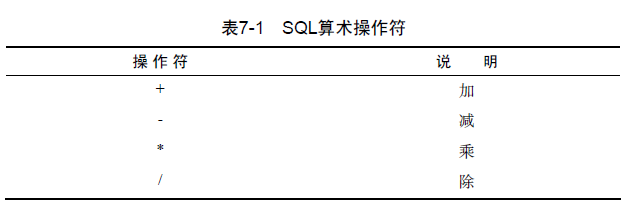
\includegraphics[width=0.8\textwidth]{3.png}
\end{figure}

\chapter{使用函数处理数据}
这一课介绍什么是函数,DBMS 支持何种函数,以及如何使用这些函数;
还将讲解为什么SQL 函数的使用可能会带来问题。
\section{函数}
\subsection{函数带来的问题}
与几乎所有DBMS 都等同地支持SQL 语句(如SELECT)不同,每一个
DBMS 都有特定的函数。事实上,只有少数几个函数被所有主要的DBMS
等同地支持。虽然所有类型的函数一般都可以在每个DBMS 中使用,但
各个函数的名称和语法可能极其不同。为了说明可能存在的问题,表8-1
列出了3 个常用的函数及其在各个DBMS 中的语法:
\begin{figure}[H]
	\centering
	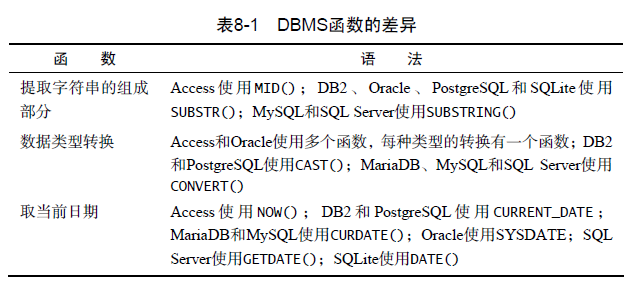
\includegraphics[width=0.8\textwidth]{4.png}
\end{figure}
可以看到,与SQL 语句不一样,SQL 函数不是可移植的。这意味着为特
定SQL 实现编写的代码在其他实现中可能不正常。
\begin{tcolorbox}[colback=blue!7!white,colframe=blue!40]
	\textbf{可移植(portable)}	
	
	所编写的代码可以在多个系统上运行。
\end{tcolorbox}

现在,你面临是否应该使用函数的选择。决定权在你,使用或是不使
用也没有对错之分。如果你决定使用函数,应该保证做好代码注释,
以便以后你(或其他人)能确切地知道所编写的SQL 代码的含义。

\section{使用函数}
大多数SQL 实现支持以下类型的函数。
\begin{itemize}
	\item 用于处理文本字符串(如删除或填充值,转换值为大写或小写)的文本函数。
	\item 用于在数值数据上进行算术操作(如返回绝对值,进行代数运算)的
	数值函数。
	\item 用于处理日期和时间值并从这些值中提取特定成分(如返回两个日期
	之差,检查日期有效性)的日期和时间函数。
	\item 返回DBMS 正使用的特殊信息(如返回用户登录信息)的系统函数。
\end{itemize}

我们在上一课看到函数用于SELECT 后面的列名,但函数的作用不仅于
此。它还可以作为SELECT 语句的其他成分,如在WHERE 子句中使用,
在其他SQL 语句中使用等,后面会做更多的介绍。

\subsection{文本处理函数}
这次使用的是UPPER()函数:
\begin{lstlisting}[language=sql]
mysql> select vend_name,upper(vend_name) as vend_name_upcase
-> from vendors
-> order by vend_name;
+----------------+------------------+
| vend_name      | vend_name_upcase |
+----------------+------------------+
| ACME           | ACME             |
| Anvils R Us    | ANVILS R US      |
| Furball Inc.   | FURBALL INC.     |
| Jet Set        | JET SET          |
| Jouets Et Ours | JOUETS ET OURS   |
| LT Supplies    | LT SUPPLIES      |
+----------------+------------------+
6 rows in set (0.01 sec)
\end{lstlisting}
可以看到,UPPER()将文本转换为大写,因此本例子中每个供应商都列
出两次,第一次为Vendors 表中存储的值,第二次作为列vend\_name\_
upcase 转换为大写。
\begin{figure}[H]
	\centering
	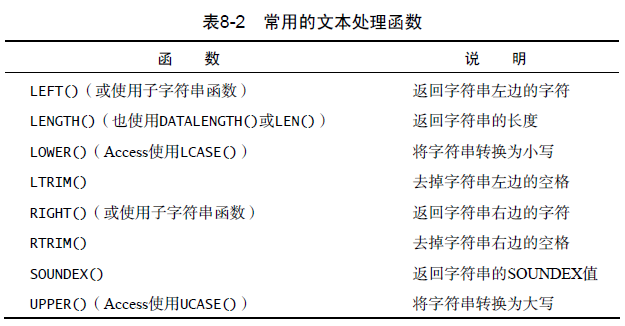
\includegraphics[width=0.8\textwidth]{5.png}
\end{figure}

表8-2 中的SOUNDEX 需要做进一步的解释。SOUNDEX 是一个将任何文
本串转换为描述其语音表示的字母数字模式的算法。SOUNDEX 考虑了
类似的发音字符和音节,使得能对字符串进行发音比较而不是字母比
较。虽然SOUNDEX 不是SQL 概念,但多数DBMS 都提供对SOUNDEX
的支持。Microsoft Access 和PostgreSQL 不支持SOUNDEX().

下面给出一个使用SOUNDEX()函数的例子。Customers 表中有一个顾客
Coyote Inc.,其联系名为Y LI。但如果这是错误的输入,
此联系名实际上应该是Y Lee ,该怎么办呢?显然,按正确的
联系名搜索不会返回数据,如下所示:
\begin{lstlisting}[language=sql]
mysql> select cust_name,cust_contact
-> from customers
->  where cust_contact='Y LI';
Empty set (0.00 sec)
\end{lstlisting}
\begin{lstlisting}[language=sql]
mysql>  select cust_name,cust_contact
->  from customers
-> where soundex(cust_contact)=soundex('Y LI');
+-------------+--------------+
| cust_name   | cust_contact |
+-------------+--------------+
| Coyote Inc. | Y Lee        |
+-------------+--------------+
1 row in set (0.00 sec)
\end{lstlisting}
\subsection{日期和时间处理函数}
日期和时间采用相应的数据类型存储在表中,每种DBMS 都有自己的特
殊形式。日期和时间值以特殊的格式存储,以便能快速和有效地排序或
过滤,并且节省物理存储空间。
应用程序一般不使用日期和时间的存储格式,因此日期和时间函数总是
用来读取、统计和处理这些值。由于这个原因,日期和时间函数在SQL
中具有重要的作用。遗憾的是,它们很不一致,可移植性最差。


\begin{lstlisting}[language=sql]
	
\end{lstlisting}
\begin{lstlisting}[language=sql]
	
\end{lstlisting}
\begin{lstlisting}[language=sql]
	
\end{lstlisting}
\begin{lstlisting}[language=sql]
	
\end{lstlisting}
\begin{lstlisting}[language=sql]
	
\end{lstlisting}
\begin{lstlisting}[language=sql]
	
\end{lstlisting}
\begin{lstlisting}[language=sql]
	
\end{lstlisting}
\begin{lstlisting}[language=sql]
	
\end{lstlisting}
\begin{lstlisting}[language=sql]
	
\end{lstlisting}

\end{document}